\section{Symmetry Breaking Using Additive $\epsilon$-costs}
\label{sec:contribution}
The TRANSIT algorithm does not appear to have been tested previously on
grid-based maps of the type commonly found in video games.
Upon a first attempt we observed the algorithm often has
prohibitively large memory requirements and relatively long query times.
This behavior can be traced to a property commonly found in grid maps but rarely in
road networks: uniform-cost path symmetries~\cite{harabor11b}.
To overcome this difficulty we propose a novel symmetry breaking technique which we
apply during preprocessing and which involves the addition of small positive ``noise''
to all edge weights.
This idea has been previously suggested in the context of symmetry breaking for
Integer Linear Programming~\cite{margot09} but the authors note that such
perturbation ``does not help much and can even be counter-productive''.
In our case, perturbation of edge weights significantly reduces the number of transit nodes and 
leads to faster preprocessing times, lower memory
requirements and significantly better query times.
To the best of our knowledge, we are the first to successfully apply such a technique
to symmetry breaking in pathfinding search.
Our idea is generally applicable to any kind of search graph; we exemplify it
on the 4-connected grid in Figure~\ref{fig:symmetry_transit}.

\begin{figure}[tb]
\centering
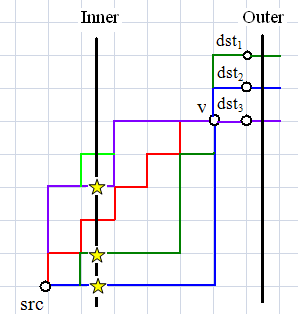
\includegraphics[height=4cm]{diagrams/symmetry_transit.PNG}
\caption{
(a) Example of many symmetric shortest paths between $src$ and $v$ in 4-connected grid network.
(b) Example of shortest paths from $src$ to $dst_1$, $dst_2$ and $dst_3$ that share many common shortest subpaths from $src$ to $v$.
}
\label{fig:symmetry_transit}
\end{figure}

Assume that during TRANSIT's preprocessing phase we are calculating shortest paths from the node $src$ to
each of $dst_1$, $dst_2$ and $dst_3$ -- which all reside on the border of the Outer square $O$.
Notice that each shortest path shares a common symmetric subpaths $src \rightsquigarrow v$ and crosses the Inner square $I$  in three  different locations.
 Therefore we identify $T_1$, $T_2$ and $T_3$ as transit nodes (starred locations in Figure~\ref{fig:symmetry_transit}). 
Our intuition is as follows: if we will add a ``small'' random $\epsilon$-cost
to each edge in the grid, there will be (with high probability)\footnote{
In practice computer representation of real numbers is finite and
commonly default to 64 bits. Assuming $b_1$ bits are required to represent the 
edges costs, and $b_2$ bits required to encode length of the longest shortest path in $G$, there are $c = 64 - b_1-b_2$ bits available to represent $\epsilon$-costs in order to preserve optimality. Therefore, probability of remaining with two different paths of length $l$ with the same perturbed weight is equivalent to the probability that we draw 2 sets of size $l$ of random numbers from $2^{c}$ numbers that sums up to the same.} only one shortest path to node $v$, e.g. through $T_{3}$.
We assume here that $src \rightsquigarrow v$ will appear as a common subpath for two or more of $dst1$, $dst2$, $dst3$; although theoretically this is not guaranteed it occurs very often in practice.

We will now show that choosing $\epsilon$ sufficiently small will preserve optimality of all shortest paths.

\begin{definition}
\label{definition:epsilon}
Let $G = (V, E)$ be a weighted graph with integer costs (if they're not integer, we just scale them up by a suitable factor so that they are) and let $L$ be the length (number of links) of the longest shortest path in $G$. Then we define $\epsilon = \frac{1}{L}$. 
\end{definition}
Note for all practical purposes there is no need to actually calculate the length of the longest shortest path $L$, but we can use $|V|$ as an upper bound.

\begin{definition}
Let $G(\epsilon)$ to be an exact copy of $G$ with the only difference that for every edge $e$ in $G(\epsilon)$ we add a
random number from the interval $(0, \epsilon)$.
\end{definition}

\begin{lemma}
\label{lemma:epsilon}
For every optimal path $\pi_{\epsilon}$ in $G(\epsilon)$
there exists a corresponding shortest path $\pi$ in $G$ that traverses
through exactly the same nodes as $\pi_{\epsilon}$.
\end{lemma}

\begin{proof}
By contradiction. Let $\pi_{\epsilon}$ in $G(\epsilon)$ be an optimal path between two nodes $src$ and $dst$.
Let $\pi$ be a path in $G$ which travels through the same nodes as $\pi_{\epsilon}$ but is not optimal.
This means there exists another path $\pi'$ between $src$ and $dst$ in $G$ which is strictly shorter than $\pi$.
Let $\pi'_{\epsilon}$ be a non-optimal path in $G_{\epsilon}$  which travels through the same nodes as $\pi'$.
Now we notice that the smallest difference between costs of any two paths in $G$ can be at least 1.
From Definition~\ref{definition:epsilon} this can only happen if $\pi'_{\epsilon}$ is longer than L, which is impossible.
\end{proof}

A natural value for L in a 4-connected grid map is $\epsilon = \frac{1}{L}$; 
for 8-connected grids we define $\epsilon = \frac{2-\sqrt{2}}{L}$.

\begin{corollary}
Number of transit nodes identified in $G(\epsilon)$ is no greater than in $G$
\end{corollary}
\begin{proof}
Similar to Lemma 1. We omit it for brevity.
\end{proof}

A direct conclusion from the latest discussion is that during the identification of transit nodes stage,
we can safely substitute $G$ with $G(\epsilon)$ and in practice 
eliminate all symmetric path segments. This will
reduce number of transit nodes, precomputation time and storage space as well as final query time.
Notice that perturbation of the graph weights in the manner described above is not specific to grid maps or
indeed to any implementation of the TRANSIT algorithm. It is a general technique for reducing
path symmetries in graphs.

\section{Efficiently Approximating Network Size}
TRANSIT's performance strongly depends on a set of preprocessing
parameters: (i) the size of each grid cell $C$ and (ii) sizes of the Inner square $I$ and Outer square $O$.
It is not clear apriori how to choose those parameters.

In this section we propose a very simple heuristic that we found useful for choosing those
parameters and quickly estimating the size of the final preprocessing data as well as percentage of
global vs. local queries.  For a given overlay grid of size $m \times m$, we count the number of
edges crossing each horizontal and vertical line of the grid.  This number gives us  an upper bound
of the number of transit nodes and allows us to tune the grid size to match available computing
resources and application requirements.  Having selected a grid size $S$ and sizes of $I$ and $O$,
for every query it is very easy to verify whether it is global or local: we just need to check if
the two nodes at hand are within local radius of each other.  Using simple random sampling we can
build a good estimate of the percentage of global vs.local queries and we can adjust our parameter
values until we achieve the desired result.  In our experience larger values for $S$, $I$ and $O$
yield a smaller number of transit nodes and require less memory but also cover a
smaller number of global queries.
